
\section{\trHomology{}与\trConnectedness}
\label{sec:homology-connectedness}

\subsection{\trConnectedComponent{}与\trHomology}
\label{subsec:connected-components-homology}

\begin{proposition}\label{thm:hm0-connected-manifold}
若 $V$ 是\trCompact\trConnected\trManifold，则 $HM_0(V;\ZZ/2)\cong\ZZ/2$。
\end{proposition}

\begin{proof}
设 $B$ 是 $C_0(f)$ 中由诸 $a_1+a_i$（$2\le i\le r$）生成的维数为 $r-1$ 的向量子空间。我们将证明，$B$ 恰好是
\[
\partial_X\colon C_1(f)\longrightarrow C_0(f)
\]
的\trImage。

\begin{figure}[htbp]
\centering
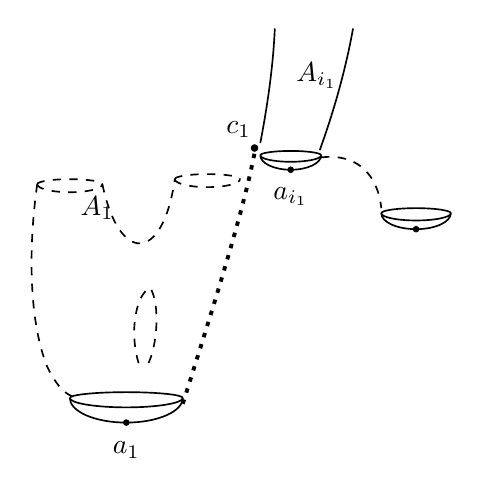
\begin{tikzpicture}[line width=0.6pt,scale=0.92]
  \draw (1.17,1.50) arc(180:360:0.78 and 0.13);
  \draw (1.17,1.50) arc(180:0:0.78 and 0.08);
  \draw (1.17,1.50) arc(180:360:0.78 and 0.34);
  \fill (1.95,1.16) circle (1.3pt);
  \node at (1.95,0.78) {$a_1$};
  \draw[dashed] (2.12,1.98) .. controls (1.98,2.45) and (2.10,2.95) .. (2.28,3.02)
                .. controls (2.42,2.80) and (2.38,2.20) .. (2.24,1.95);
  \draw[dashed] (0.72,4.45) arc(180:360:0.45 and 0.11);
  \draw[dashed] (0.72,4.45) arc(180:0:0.45 and 0.07);
  \draw[dashed] (2.62,4.52) arc(180:360:0.45 and 0.11);
  \draw[dashed] (2.62,4.52) arc(180:0:0.45 and 0.07);
  \draw[dashed] (1.62,4.45) .. controls (1.85,3.35) and (2.45,3.35) .. (2.62,4.52);
  \draw[dashed] (0.72,4.45) .. controls (0.60,3.60) and (0.60,2.60) .. (0.85,1.95)
                .. controls (1.00,1.62) and (1.17,1.50) .. (1.30,1.50);
  \node at (1.55,4.12) {$A_1$};
  \draw[line width=1.4pt,dash pattern=on 1.6pt off 2.6pt]
    (2.73,1.42) .. controls (3.10,2.60) and (3.55,4.00) .. (3.72,4.88);
  \fill (3.72,4.95) circle (1.5pt);
  \node at (3.50,5.20) {$c_1$};
  \draw (3.80,4.85) arc(180:360:0.42 and 0.09);
  \draw (3.80,4.85) arc(180:0:0.42 and 0.06);
  \draw (3.80,4.85) arc(180:360:0.42 and 0.20);
  \fill (4.22,4.65) circle (1.3pt);
  \node at (4.22,4.28) {$a_{i_1}$};
  \draw (3.80,5.02) .. controls (3.92,5.65) and (3.98,6.15) .. (4.00,6.60);
  \draw (4.62,4.92) .. controls (4.85,5.55) and (5.00,6.15) .. (5.08,6.60);
  \node at (4.58,5.95) {$A_{i_1}$};
  \draw[dashed] (4.64,4.82) .. controls (5.12,4.88) and (5.42,4.60) .. (5.47,4.12);
  \draw (5.47,4.05) arc(180:360:0.48 and 0.10);
  \draw (5.47,4.05) arc(180:0:0.48 and 0.07);
  \draw (5.47,4.05) arc(180:360:0.48 and 0.22);
  \fill (5.95,3.83) circle (1.3pt);
\end{tikzpicture}
\caption{}
\label{fig:n-basins}
\end{figure}

我们先来证明 $\partial_XC_1\subset B$，这是容易的那个包含关系。设 $c$ 是一个\trIndex{}为 1 的\trCriticalPoint。它的\trUnstableManifold{}的维数是 1，因此自 $c$ 出发的 $X$ 的\trTrajectory{}只有两条。这两条分别到达两个局部极小点 $a_i$ 与 $a_j$（二者未必不同）。于是我们有
\[
\partial_Xc=a_i+a_j=(a_1+a_i)+(a_1+a_j)\in B\text{。}
\]
从而 $\partial_X(C_1(f))\subset B$。

反过来，我们来证明 $B\subset\partial_X(C_1(f))$（这是证明的核心部分）。只需证明：对每个 $i$，$a_i$ 与 $a_1$ 属于同一个\trHomology{}类。令
\[
N=V-\bigcup_{\operatorname{Ind}(x),\operatorname{Ind}(y)\ge 2}\mathcal{M}(x,y)\text{。}
\]
注意，在 $\operatorname{Ind}(x)$、$\operatorname{Ind}(y)\ge 2$ 的条件下，我们有 $\operatorname{codim}\mathcal{M}(x,y)\ge 2$，故 $N$ 是\trConnected{}的。对 $j=1,\dotsc,r$，我们令
\[
A_j=\bigl\{\,x\in N \mid x \text{ 位于某条终止于 } a_j \text{ 的（破碎）\trTrajectory{}上}\,\bigr\}\text{。}
\]
诸 $A_j$ 都是\trConnected{}的（$A_j$ 的所有点都与 $a_j$ 相\trConnected），$N$ 是诸 $A_j$ 的并，而 $A_j$ 则是 $a_j$ 的\trStableManifold{}与那些终止于 $a_j$ 且经过一个\trIndex{}为 1 的\trCriticalPoint{}的\trTrajectory{}之并。\cref{fig:n-basins}展示了 $N$ 的一部分，以及与之相应的 $A_1$ 与 $A_{i_1}$ 的部分。

现在我们来证明诸 $A_j$ 都是 $N$ 的\trClosed{}子集。只需对 $j=1$ 证明此事。设 $(x_n)$ 是 $A_1$ 中一个\trConvergence{}到 $x\in N$ 的序列。我们将证明 $x\in A_1$。我们假定诸 $x_n$ 都不是 $f$ 的\trCriticalPoint，这对我们的需要来说已经足够。设 $\ell_n$ 是过 $x_n$ 的那条\trTrajectory，而 $\ell$ 是过 $x$ 的那条。在必要时抽取一个子列之后，我们可以——而且我们也确实——假定诸\trTrajectory{} $\ell_n$ 全都终止于同一个\trCriticalPoint{} $b$；这个 $b$ 可以是 $a_1$，也可以是另一个\trIndex{}为 1 的\trCriticalPoint——它本身有一条\trTrajectory{}通到 $a_1$。

设 $c$ 是 $\ell$ 所到达的那个\trCriticalPoint。由于 $x$ 属于 $N$，它的\trIndex{}为 0 或 1。若 $c=b$，那么证明就完成了。否则，设 $\ell^+$ 为 $\ell$ 进入 $c$ 的\trMorseChart{}时所经过的那个点。由解对初始条件的连续性，诸 $\ell_n$ 也进入这张\trChart。设 $\ell_n^+$ 为 $\ell_n$ 的进入点。根据\cref{thm:same-level-convergence}，诸 $\ell_n^+$ 构成的序列趋于 $\ell^+$。由于我们已经假定 $c\neq b$，诸\trTrajectory{} $\ell_n$ 便经由一些点 $\ell_n^-$ 离开这张\trChart。仍根据\cref{thm:same-level-convergence}，从序列 $(\ell_n^-)$ 中抽出的一个\trConvergence{}子列的极限是某个 $\lambda^-\in W^u(c)$（正如\cref{thm:broken-space-compact}的证明中那样）。$\lambda^-$ 的\trTrajectory{} $\lambda$ 把 $c$ 与一个必定\trIndex{}为 0 的\trCriticalPoint{} $a$ 连接起来。由于诸 $\ell_n$ 在 $n$ 充分大时都进入 $a$ 的\trMorse{}邻域，我们必有 $a=a_1$（$=b$）以及 $x\in A_1$。故 $A_1$ 是 $N$ 的一个\trClosed{}子集。

由于 $N$ 是\trConnected{}的，存在一个\trIndex{} $i_1>1$ 使得 $A_1\cap A_{i_1}\neq\varnothing$。这个交必定含有一个\trIndex{}为 1 的\trCriticalPoint，设为 $c_1$。我们有
\[
\partial_Xc_1=a_1+a_{i_1}\text{，}
\]
于是 $a_{i_1}$ 与 $a_1$ 属于同一个\trHomology{}类。此外，$A_1\cup A_{i_1}$ 是\trConnected{}的。因此存在一个\trIndex{} $i_2$ 使得 $(A_1\cup A_{i_1})\cap A_{i_2}\neq\varnothing$。这个交含有来自某个\trIndex{}为 1 的\trCriticalPoint{} $c_2$ 的一条\trTrajectory，于是我们有
\[
\partial_Xc_2=a_1+a_{i_2}\qquad\text{或}\qquad\partial_Xc_2=a_{i_1}+a_{i_2}\text{。}
\]
在这两种情形下，$a_{i_2}$ 的\trHomology{}类都与 $a_1$ 的相同。我们重复这一论证，直到不再剩下任何 $a_i$ 为止，这就表明它们全都\trHomology{}于 $a_1$。
\end{proof}

\begin{remark}\label{thm:proof-dim1-analogous}
这个证明与我们在对维数 1 的\trManifold{}进行分类时所用的那个证明（\cref{subsec:classification-theorem}小节）完全类似。
\end{remark}

应用\trPoincareDuality，我们从\cref{thm:hm0-connected-manifold}推出下面的结果。

\begin{corollary}\label{thm:hmn-connected-manifold}
设 $V$ 是维数为 $n$ 的\trCompact\trConnected\trManifold；那么 $HM_n(V;\ZZ/2)\cong\ZZ/2$。\noqed
\end{corollary}

\begin{remark}\label{thm:hm-z-oriented}
\cref{thm:hm0-connected-manifold}在 $\ZZ$ 上也成立，这只需在证明中对诸\trOrientation{}多加留意便可看出。\cref{thm:hmn-connected-manifold}的类似结论于是便是：若 $V$ 是维数为 $n$ 的\trCompact\trConnected\trOrientation\trManifold，则 $HM_n(V;\ZZ)\cong\ZZ$。
\end{remark}

\begin{corollary}\label{thm:hm0-hmn-components}
设 $V$ 是维数为 $n$ 的\trCompact\trManifold。那么 $HM_0(V;\ZZ/2)$ 与 $HM_n(V;\ZZ/2)$ 都是 $\ZZ/2$-\trVectorSpace，其维数等于 $V$ 的\trConnectedComponent{}的个数。
\end{corollary}

\begin{proof}
我们把 $V$ 写成其诸\trConnectedComponent{}的\trDisjointUnion：
\[
V=\coprod_{i=1}^{k}V_i\text{。}
\]
在每个 $V_i$ 上，我们选一个\trMorseFunction{} $f_i$ 与一个\emph{合适}的\trVectorField{} $X_i$。显然有
\[
C_*\Bigl(\coprod f_i\Bigr)=\bigoplus C_*(f_i)\qquad\text{与}\qquad
  \partial_{\coprod X_i}=\bigoplus\partial_{X_i}\text{，}
\]
这就给出了结果。
\end{proof}

\begin{remark}\label{thm:unique-local-minimum}
\cref{thm:hm0-connected-manifold}的证明还告诉我们：\trCompact\trConnected\trManifold{}上一个没有\trIndex{}为 1 的\trCriticalPoint{}的\trMorseFunction{}具有唯一的局部极小点；这个结果在\trSymplectic{}几何的一个著名定理——Atiyah--Guillemin--Sternberg 凸性定理——的证明中是必不可少的（例如参见~[5]~以及那里所引的原始文献）。
\end{remark}

\subsection{\trFundamentalGroup{}与\trHomology{}（第一部分）}
\label{subsec:fundamental-group-homology-1}

沿着同样的思路，并且不真正用到\trMorseComplex，我们来开始比较（\trConnected{}）\trManifold{} $V$ 的\trFundamentalGroup{}与第一\trHomology{}群。最理想的结果本应是：$HM_1(V;\ZZ)$ 是群 $\pi_1(V)$ 的最大\trAbelianGroup{}商。\footnote{译注：即 $\pi_1(V)$ 的阿贝尔化（abelianization）。}事实也确实如此。我们稍后（在\cref{subsec:fundamental-group-homology-2}小节中）将证明一个较弱的结果：若 $V$ 是\trSimplyConnected{}的，则 $HM_1(V;\ZZ)$ 为零。眼下，我们只满足于指出下面的结果。

\begin{proposition}\label{thm:no-index-one-simply-connected}
若\trManifold{} $V$ 容许一个没有\trIndex{}为 1 的\trCriticalPoint{}的\trMorseFunction，则它是\trSimplyConnected{}的。\footnote{译注：原书陈述即如此，照排于此；按字面本命题缺少\trCompact{}（无边界）前提，实为假：取非\trCompact{}的 $V=S^1\times\RR$ 与 $f(\theta,t)=t$，则 $f$ 没有任何\trCriticalPoint{}（遑论\trIndex{}为 1 者），而 $\pi_1(V)\cong\ZZ$ 非平凡；补上“$V$ \trCompact{}（无边界）\trConnected{}”的前提后，上述证明方能成立。——译者注}
\end{proposition}

\begin{proof}
我们可以——而且我们也确实——假定 $V$ 是道路\trConnected{}的，并选取 $f$ 的一个极小点（比如说 $a_0$）作为基点。设 $C$ 是 $V$ 中的一个\trLoop。我们可以——而且我们也确实——假定这个\trLoop{}是可微的。若 $b$ 是一个\trIndex{}为 $k$ 的\trCriticalPoint，那么我们知道 $\dim W^s(b)=n-k$。由一个一般位置论证，我们可以——而且我们也确实因此——假定 $C$ 不与任何\trIndex{}大于或等于 2 的\trCriticalPoint{}的\trStableManifold{}相交。既然我们已经假定不存在\trIndex{}为 1 的\trCriticalPoint，\trLoop{} $C$ 就包含于诸局部极小点的\trStableManifold{}的并之中，而这些\trStableManifold{}两两不相交。因此 $C$ 包含于其中一个\trStableManifold{}之内，即 $a_0$ 的那一个。但后者是一个\trDisk，在这个\trDisk{}里把 $C$ 收缩到基点 $a_0$ 上毫无困难。
\end{proof}

\begin{example}\label{thm:sphere-simply-connected}
例如，\trSphere{} $S^n$ 只要 $n\ge 2$ 就是\trSimplyConnected{}的。
\end{example}
